\section{The revised prototypes}
We inherited a set of power-point slides from the last year's product owner group.
This was a large collection of 122 slides that was not interactable. 
Some of these slides were also not visually acceptable, leading to us making the decision of redoing the prototypes.
As described in the LABEL TECHNOLOGY, Adobe XD was used to create a new design and allow for interaction in the design.
By the prototypes being interactable, it is meant that users can click on certain areas and transitions will occur to illustrate the functionality.
\todo{LABEL TECHNOLOGIES USED AND REF HERe}
Some of the updated prototypes will be compared to the previous versions in the following section.

\subsection{The login screen and choosing citizen}
The base design of the previous login screen was functinoally acceptable. 
The background color used was just a dull yellow, and as such updated the background to be a little more dynamic but keeping the separate bars in which to input username and password.
A comparison of the screen in which a citizen is illustrated in the following figure:
\begin{figure}[h]
 
    \begin{subfigure}{0.5\textwidth}
    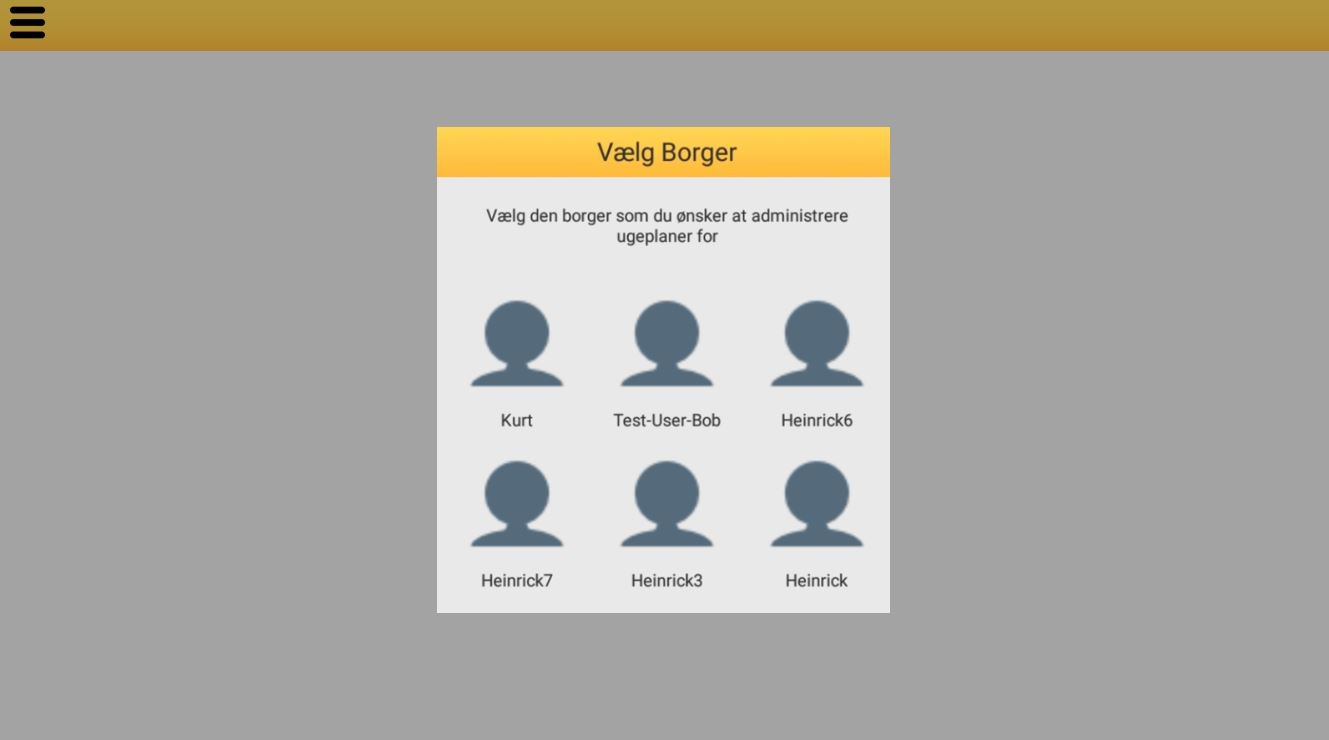
\includegraphics[width=0.9\linewidth, height=5cm]{previous_citizen_select.JPG} 
    \caption{The previous citizen select screen}
    \label{fig:previous_citizen_select}
    \end{subfigure}
    \begin{subfigure}{0.5\textwidth}
    
    \caption{The proposed new select screen}
    \label{fig:new_citizen_select}
    \end{subfigure}
     
    \caption{This figure shows both citizen select screens}
    \label{fig:citizen_select}
    \end{figure}

\begin{figure}[]
    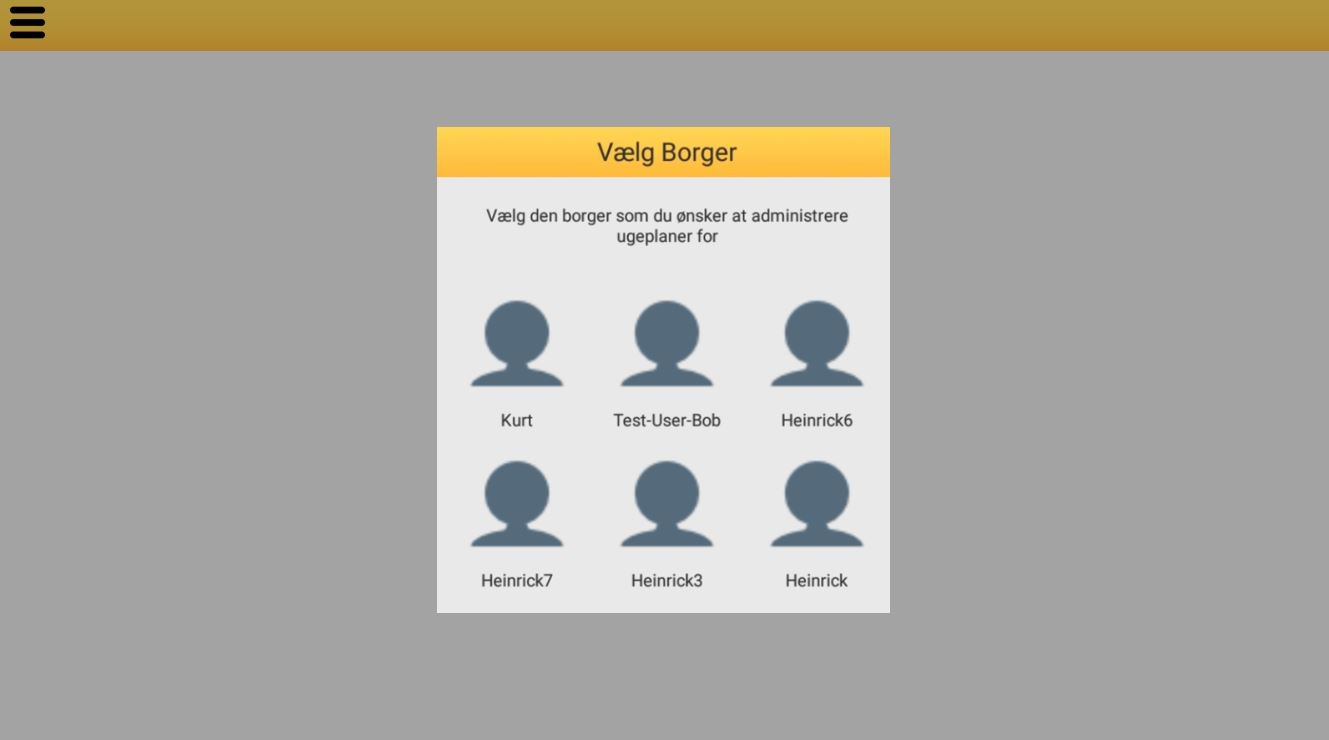
\includegraphics[width=0.5\textwidth]{previous_citizen_select.JPG}
    \caption{The previous citizen select screen}
\end{figure}
